% !TeX root = ../main.tex
\chapter{视觉里程计}
视觉SLAM主要分为视觉前端和后端优化。前端也称为视觉里程计,这是通过相邻图像间的信息估计出粗略的相机运动,给后端提供较好的初始值。视觉里程计的实现也分几种,按照是否需要提取特征,分为特征点法的前端和不提取特征点的直接法前端。基于特征点法的前端被认为是较好的方法,它运行稳定,对光照、动态物体不敏感,是目前比较成熟的解决方案。通过前几章的技术积累,我们已经初步具备了设计一个视觉里程计的能力。\par
\section{单目SLAM的初始化}
对于单目SLAM来说,存在一个尺度问题。我们知道对极几何满足这样的关系:
\begin{equation}
\hat{\boldsymbol{x}}_2^T\left[\boldsymbol{t}\right]_{\times}\boldsymbol{R}\hat{\boldsymbol{x}}_1=0
\end{equation}
可以看到,在方程两边同时乘以某个常数,方程仍然成立。这就意味着从本质矩阵E估计出的t是不可靠的。所以我们并不能连续计算两幅相邻的图片去估计相机的位姿。那解决这个问题的方法就是对前两幅图片的$\boldsymbol{t}$进行归一化,后续的图片通过PnP(后面会介绍)来计算R和t。在单目视觉中,我们对初始两张图像的$\boldsymbol{t}$归一化相当于固定了尺度。虽然我们并不知道$\boldsymbol{t}$的单位是多少,但是我们可以以前两幅图的移动为单位1,以此计算特征点的3D位置。由以上描述我们也可以知道,前两幅图的位置关系不能是纯旋转。纯旋转的两张图无法进行初始化。
\section{三角测量}
\begin{figure}[H]
	\centering
	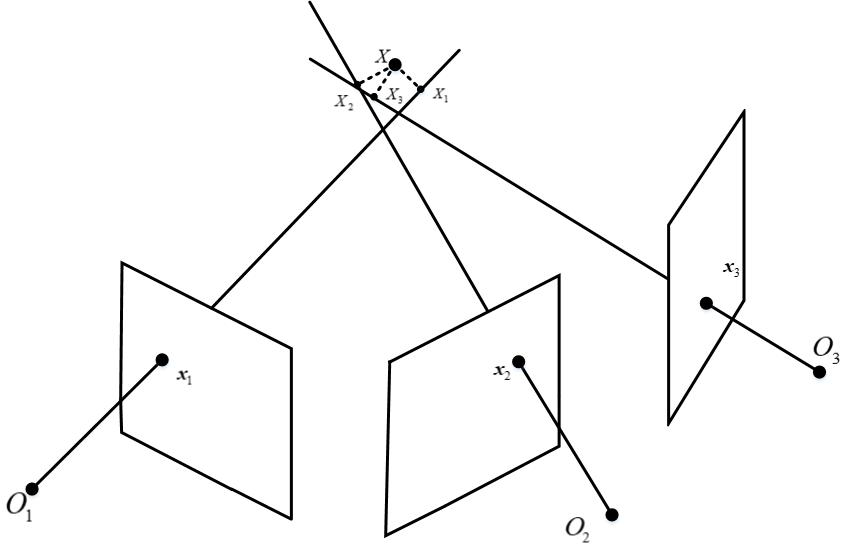
\includegraphics[height=5cm]{triangulation}
	\caption{三角化}
	\label{fig:triangulation}
\end{figure}
假如我们设$x_1,x_2$为两个特征点的归一化坐标,那么他们满足:
\begin{equation}
	s_1\boldsymbol{x_1}=s_2\boldsymbol{Rx_2}+\boldsymbol{t}
\end{equation}
现在我们已经解得$\boldsymbol{R},\boldsymbol{t}$,想要求解出$s_1,s_2$。以求解$s_2$为例,先在两边叉乘一个$x_1$:
\begin{equation}
s_1\left[\boldsymbol{x_1}\right]_{\times}\boldsymbol{x_1}=0=s_2\left[\boldsymbol{x_1}\right]_{\times}\boldsymbol{Rx_2}+\left[\boldsymbol{x_1}\right]_{\times}\boldsymbol{t}
\end{equation}
式子左侧为0,右边的R和t以及$x_1,x_2$都是已知的,由此求得$s_2$。OpenCV中提供了cv::triangulatePoints()函数来实现三角测量。
\section{PnP方法}
上面提到,在求解后面的图片的时候,并不会用到分解本质矩阵得到$R,t$的方法来定位,而是采用PnP(Perspective-n-Point)求解。PnP是求解3D到2D点对的方法。当我们知道n个3D空间点的位置及其投影位置时,如何估计相机位姿。如果两张图像中的一张特征点3D位置已知,那么至少需要3个点对就可以估计相机运动。这种3D-2D方法不需要用到对极约束,又可以在很少的匹配点中获得较好的运动估计,是一种最重要的姿态估计方法。\par
PnP的求解方法有很多种,P3P\cite{gao2003complete}、直接线性变换(DLT)、EPnP\cite{lepetit2009epnp}、UPnP\cite{penate2013exhaustive}等。也可以用非线性优化的方式求解,也就是Bundle Adjustment。
\subsection{直接线性变换}
考虑某个空间点P,它的齐次坐标为$\boldsymbol{P}=(X, Y, Z, 1)^{\mathrm{T}}$,在图像$I_1$中,投影到特征点$x_{1}=\left(u_{1}, v_{1}, 1\right)^{\mathrm{T}}$((归一化平面)。我们已知的是P和特征点$x_1$,R和t为未知。与求解本质矩阵相似,我们可以定义一个增广矩阵$\left[\boldsymbol{R} | \boldsymbol{t}\right]$为一个3$\times$4的矩阵:
\begin{equation}
s \left( \begin{array}{c}{u_{1}} \\ {v_{1}} \\ {1}\end{array}\right)=\left( \begin{array}{cccc}{t_{1}} & {t_{2}} & {t_{3}} & {t_{4}} \\ {t_{5}} & {t_{6}} & {t_{7}} & {t_{8}} \\ {t_{9}} & {t_{10}} & {t_{11}} & {t_{12}}\end{array}\right) \left( \begin{array}{l}{X} \\ {Y} \\ {Z} \\ {1}\end{array}\right)
\end{equation}
显然$s=t_{9} X+t_{10} Y+t_{11} Z+t_{12}$,消去s得:
\begin{equation}
u_{1}=\frac{t_{1} X+t_{2} Y+t_{3} Z+t_{4}}{t_{9} X+t_{10} Y+t_{11} Z+t_{12}}, \quad v_{1}=\frac{t_{5} X+t_{6} Y+t_{7} Z+t_{8}}{t_{9} X+t_{10} Y+t_{11} Z+t_{12}}
\end{equation}
为了简化表示,定义一个T向量:
\begin{equation}
t_{1}=\left(t_{1}, t_{2}, t_{3}, t_{4}\right)^{\mathrm{T}}, t_{2}=\left(t_{5}, t_{6}, t_{7}, t_{8}\right)^{\mathrm{T}}, t_{3}=\left(t_{9}, t_{10}, t_{11}, t_{12}\right)^{\mathrm{T}}
\end{equation}
于是关于$u_1,v_1$的方程可表示为:
\begin{equation}
\begin{array}{l}{t_{1}^{\mathrm{T}} \boldsymbol{P}-\boldsymbol{t}_{3}^{\mathrm{T}} \boldsymbol{P} u_{1}=0} \\ {\boldsymbol{t}_{2}^{\mathrm{T}} \boldsymbol{P}-\boldsymbol{t}_{3}^{\mathrm{T}} \boldsymbol{P} v_{1}=0}\end{array}
\end{equation}
可以看到,每个特征点能够提供两个约束,假设一共有N个特征点,可列出如下方程:
\begin{equation}
\left(\begin{array}{ccc}
{\boldsymbol{P}_{1}^{\mathrm{T}}} & {0} & {-u_{1} \boldsymbol{P}_{1}^{\mathrm{T}}} \\ {0} & {\boldsymbol{P}_{1}^{\mathrm{T}}} & {-v_{1} \boldsymbol{P}_{1}^{\mathrm{T}}} \\ {\vdots} & {\vdots} & {\vdots} \\ {\boldsymbol{P}_{N}^{\mathrm{T}}} & {0} & {-u_{N} \boldsymbol{P}_{N}^{\mathrm{T}}} \\ {0} & {\boldsymbol{P}_{N}^{\mathrm{T}}} & {-v_{N} \boldsymbol{P}_{N}^{\mathrm{T}}}
\end{array}\right)\left( \begin{array}{l}{t_{1}} \\ {t_{2}} \\ {t_{3}}\end{array}\right)=0
\end{equation}
当N=6时,恰有解析解。当N>6时,可采用SVD分解来求取超静定方程最小二乘解。\par
但这样的解法只是假设了十二个未知数,并没有约束。但是R需要是正交矩阵,DLT的结果不一定满足要求,这时我们就需要寻找一个最好的旋转矩阵当做它的近似解。也就是对DLT的结果做QR分解。
\subsection{非线性优化(BA)}
除了上面介绍的DLT方法之外,我们还可以把PnP问题构建成一个定义于李代数上的非线性最小二乘问题。前面说的方法基本是先求相机位姿,再求空间点的位置,而BA将其都看成优化变量。也就是说BA过程中相机的位姿和空间点的位置都会同步优化,以求得最符合的结果。我们这里的BA问题是一个最小化重投影误差的过程。\par
我们设一空间点$P_i$的齐次坐标为$\boldsymbol{P}_i=(X, Y, Z, 1)^{\mathrm{T}}$,其投影的像素坐标是的坐标是$\boldsymbol{u_i}=(u_i, v_i)$,相机内参矩阵为K,位姿的李代数表示为$\xi$(六维向量)。我们可以定义误差函数:
\begin{equation}
\begin{aligned}
loss(\xi)=\arg \min _{\xi} \frac{1}{2} \sum_{i=1}^{n}\left\|e(\xi)\right\|_{2}^{2}\\
e(\xi)=u_{i}-\frac{1}{s_{i}} K \exp \left(\xi^{\wedge}\right) P_{i}
\end{aligned}
\label{equ:ba}
\end{equation}
这个误差项定义的是十分直观的,它表示用空间点经过位姿变换再经过相机内参投影到像素平面的坐标和原始的像素坐标的二范数。公式中隐含着一些齐次坐标转换不再一一指出。\par
那么接下来就是要考虑李代数的六个维度,该如何调整才能让误差函数$e(\xi)$达到最小。
\subsubsection{非线性优化基本思想}
我们先来考虑一个简单的最小二乘问题:
\begin{equation}
	\min_{x}\frac{1}{2}\left\|f(\boldsymbol{x})\right\|_{2}^{2}
\end{equation}
这里自变量$x \in R^n$,f是任意非线性函数。
如果f是个形式简单的函数,那么这个问题可以直接求出解析解。直接令导函数为0,解得x的最值即可。
\begin{equation}
	\frac{df}{d\boldsymbol{x}}=0
\end{equation}
解此方法即可,至于是极大值还是极小值或是鞍点只需要比较函数值即可。\par
对于不方便直接求解的最小二乘问题,我们能够用迭代的方式来计算。赋给$\boldsymbol{x}$一个初值,然后不断的更新这个变量,使目标函数下降。步骤如下:\par
\begin{enumerate}[(a)]
	\item 给定某个初值$\boldsymbol{x}_0$
	\item 对于第k次迭代,寻找一个增量$\Delta x_k$,使得$\left\|f(\boldsymbol{x}_k+\Delta \boldsymbol{x}_k)\right\|_{2}^{2}$达到极小值。
	\item 如果$\Delta \boldsymbol{x}_k$足够小,就停止迭代。
	\item 否则令$\boldsymbol{x}_{k+1}=\boldsymbol{x}+\Delta \boldsymbol{x}_k$,重复第2步。
\end{enumerate}
这个问题的关键是$\Delta \boldsymbol{x}_k$如何确定。下面介绍两种常见的方法。
\subsubsection{一阶梯度二阶梯度}
我们将目标函数在x附近做泰勒展开:
\begin{equation}
\|f(x+\Delta x)\|_{2}^{2} \approx\|f(x)\|_{2}^{2}+\boldsymbol{J}(x) \Delta x
+ \frac{1}{2}\Delta x^T \boldsymbol{H}\Delta x
\end{equation}
这里的$\boldsymbol{J}$是目标函数关于x的导数,是一个雅克比矩阵。而$\boldsymbol{H}$是二阶导数,也就是海塞(Hessian)矩阵。我们可以选择保留一阶导数或者二阶导数。如果保留一阶导数,将增量方程对$\Delta x$求导,解得:
\begin{equation}
	\Delta x = J^T(x)
\end{equation}
如果保留二阶导数,将增量方程对$\Delta x$求导,解得:
\begin{equation}
	\boldsymbol{H}\Delta x=-\boldsymbol{J}^T
\end{equation}
这里对矩阵求导涉及到了矩阵论的知识,不表。\par
保留一阶导数的方法叫做最速下降法,保留二阶导数的方法叫牛顿法。公式所表示的意义很直观,只要把函数在初值附近泰勒展开,然后一步步的在附近搜索就可以了。但是这样做也存在问题。
\begin{enumerate}[(a)]
	\item 对于保留一阶导数的情况,这样的下降方法过于贪心,容易走出锯齿形路线,找到局部最优解的速度慢。
	\item 对于保留二阶导数的情况,海塞矩阵计算量大,应当尽量避免计算海塞矩阵。
\end{enumerate}\par
\begin{figure}[H]
	\centering
	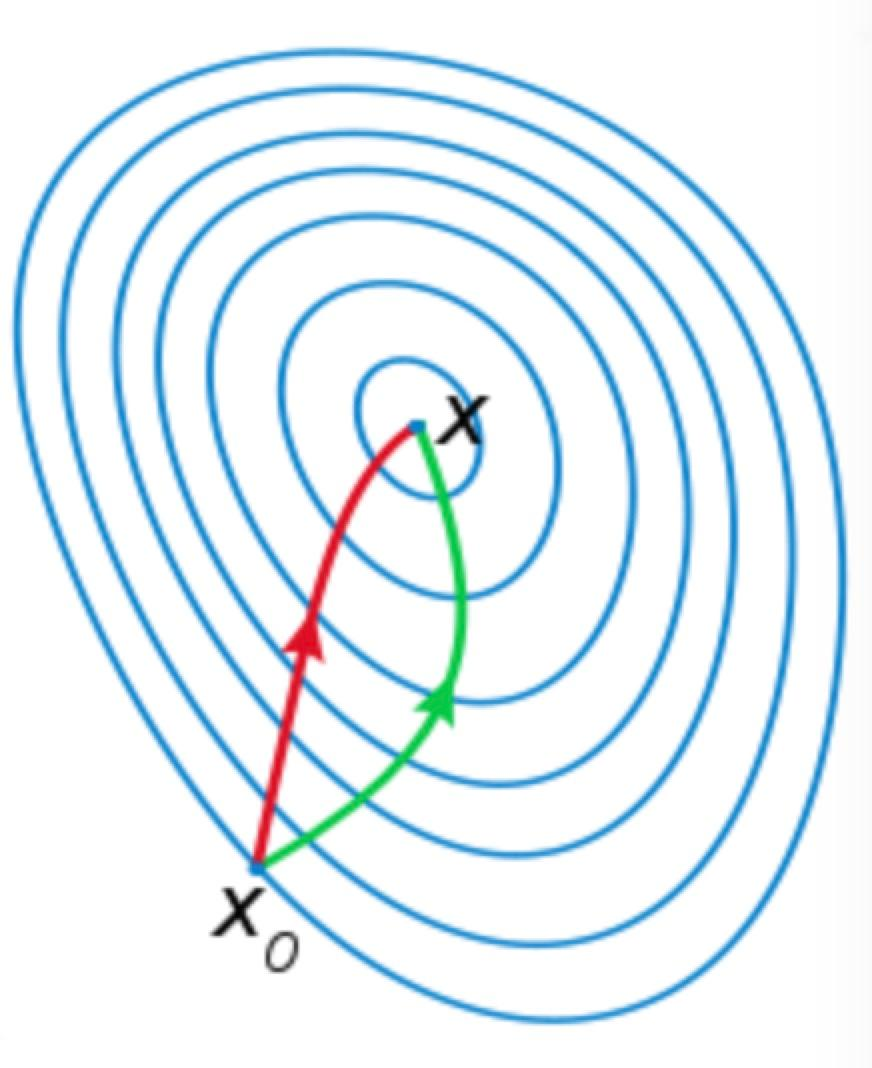
\includegraphics[height=5cm]{yijieerjie}
	\caption{红色:牛顿法 绿色:最速下降}
\end{figure}
因此可以选用另外两种更实用的方法。
\subsubsection{高斯牛顿法}
高斯牛顿法是最优化算法中比较简单的一类。我们假设目标函数$f(x)$在x处泰勒展开:
\begin{equation}
f(\boldsymbol{x}+\Delta \boldsymbol{x}) \approx f(\boldsymbol{x})+\boldsymbol{J}(\boldsymbol{x}) \Delta \boldsymbol{x}
\end{equation}
这样就在形式上跟式\ref{equ:ba}统一了,计算结果都是一个向量。我们现在计算其二范数:
\begin{equation}
e(\Delta x)=\arg \min _{\Delta x} \frac{1}{2}\|f(x)+J(x) \Delta x\|^{2}
\end{equation}
我们需要对$\Delta x$进行求导,在求导之前我们先将其展开:
\begin{equation}
\begin{aligned}
\frac{1}{2}\|f(x)+J(x) \Delta x\|^{2}=&\frac{1}{2}(f(\boldsymbol{x})+\boldsymbol{J}(\boldsymbol{x}) \Delta \boldsymbol{x})^{\mathrm{T}}(f(\boldsymbol{x})+\boldsymbol{J}(\boldsymbol{x}) \Delta \boldsymbol{x})\\
=&\frac{1}{2}\left(\|f(\boldsymbol{x})\|_{2}^{2}+2 f(\boldsymbol{x})^{\mathrm{T}} \boldsymbol{J}(\boldsymbol{x}) \Delta \boldsymbol{x}+\Delta \boldsymbol{x}^{\mathrm{T}} \boldsymbol{J}(\boldsymbol{x})^{\mathrm{T}} \boldsymbol{J}(\boldsymbol{x}) \Delta \boldsymbol{x}\right)
\end{aligned}
\end{equation}
然后再求导,令导函数为0:
\begin{equation}
2 \boldsymbol{J}(x)^{\mathrm{T}} f(\boldsymbol{x})+2 \boldsymbol{J}(\boldsymbol{x})^{\mathrm{T}} \boldsymbol{J}(\boldsymbol{x}) \Delta \boldsymbol{x}=\mathbf{0}
\end{equation}
化简后得:
\begin{equation}
J(x)^{\mathrm{T}} J(x) \Delta x=-J(x)^{\mathrm{T}} f(x)
\end{equation}
由于此方程求解的结果是增量$\Delta x$,因此我们称该方程为增量方程。定义左边系数为$\boldsymbol{H}$,定义右边系数矩阵为$\boldsymbol{g}$,那么就变成:
\begin{equation}
\boldsymbol{H} \Delta x=\boldsymbol{g}
\end{equation}
我们可以把$J^{\mathrm{T}} \mathrm{J}$理解为对$\boldsymbol{H}$的近似,从而省略了计算海塞矩阵的过程。因此,我们利用高斯牛顿法迭代的流程就是:
\begin{enumerate}[(a)]
	\item 给定初值$\boldsymbol{x}_0$
	\item 对于第k次迭代,求出当前的雅克比矩阵$J(x_k)$和误差$f(x_k)$
	\item 求解增量方程$\boldsymbol{H} \Delta x=\boldsymbol{g}$
	\item 若$\Delta x$足够小则停止,否则令$\boldsymbol{x}_{k+1}=\boldsymbol{x}+\Delta \boldsymbol{x}_k$,重复第2步。
\end{enumerate}\par
对于雅克比矩阵$\boldsymbol{J}(x_k)$和函数$f(x_k)$的求解是十分简单的,只需要带入x值就可以了。而求解$\boldsymbol{H}$是十分困难的。人们曾经一度认为由于求解H的复杂性,这种优化方法不能应用于SLAM系统,但是后来人们认识到了H的稀疏性,才使得求解大规模的增量方程成为可能。这种方法有一个问题,当通过增量方程求解出来的$\Delta x$过大的时候,就不满足泰勒展开的要求,这样一来就不能保证迭代收敛,甚至误差变的更大也有可能。列文伯格-马夸尔特(LM)方法一定程度上修正了这些问题,在SLAM里也广为应用。
\subsubsection{列文伯格-马夸尔特(LM)法}
上一节提到,高斯牛顿法当$\Delta x$过大的时候,可能会出现一些问题,甚至按照这个梯度走下去误差函数反而会增大。由此我们很自然的想到,设置一个信赖区域,当$\Delta x$小于某个值的时候,就认为高斯牛顿法是可靠的,反之则不可靠。我们考虑这样定义信赖区域:
\begin{equation}
\rho=\frac{f(\boldsymbol{x}+\Delta \boldsymbol{x})-f(\boldsymbol{x})}{\boldsymbol{J}(\boldsymbol{x}) \Delta \boldsymbol{x}}
\end{equation}
也就是当实际增量和求导计算的增量比较接近的时候,认为泰勒近似的比较好,反之则调整范围,也就是:
\begin{equation}
\min _{\Delta \boldsymbol{x}_{k}} \frac{1}{2}\left\|f\left(\boldsymbol{x}_{k}\right)+\boldsymbol{J}\left(\boldsymbol{x}_{k}\right) \Delta \boldsymbol{x}_{k}\right\|^{2}, \quad \text { s.t. }\left\|D \Delta x_{k}\right\|^{2} < \mu
\end{equation}
我们设置了信赖区域$\mu$,也就是把问题变成了一个有约束的优化问题。我们可以引入拉格朗日乘子将其重新变成无约束问题:
\begin{equation}
\min _{\Delta x_{k}} \frac{1}{2}\left\|f\left(x_{k}\right)+J\left(x_{k}\right) \Delta x_{k}\right\|^{2}+\frac{\lambda}{2}\|D \Delta x\|^{2}
\end{equation}
这里的$\lambda$是拉格朗日算子,$\boldsymbol{D}$可以看做单位阵$\boldsymbol{I}$,上式对$\Delta x$求导,相当于求解:
\begin{equation}
(H+\lambda I) \Delta x=g
\end{equation}
当参数$\lambda$较小时,$\boldsymbol{H}$占主要地位,此方法更接近高斯牛顿法,当参数$\lambda$较大时,此方法更接近最速下降法。总之,LM方法能够提供更稳定,更准确的$\Delta x$













